\documentclass{standalone}
\usepackage{tikz}
\usetikzlibrary{patterns, positioning}


\begin{document}
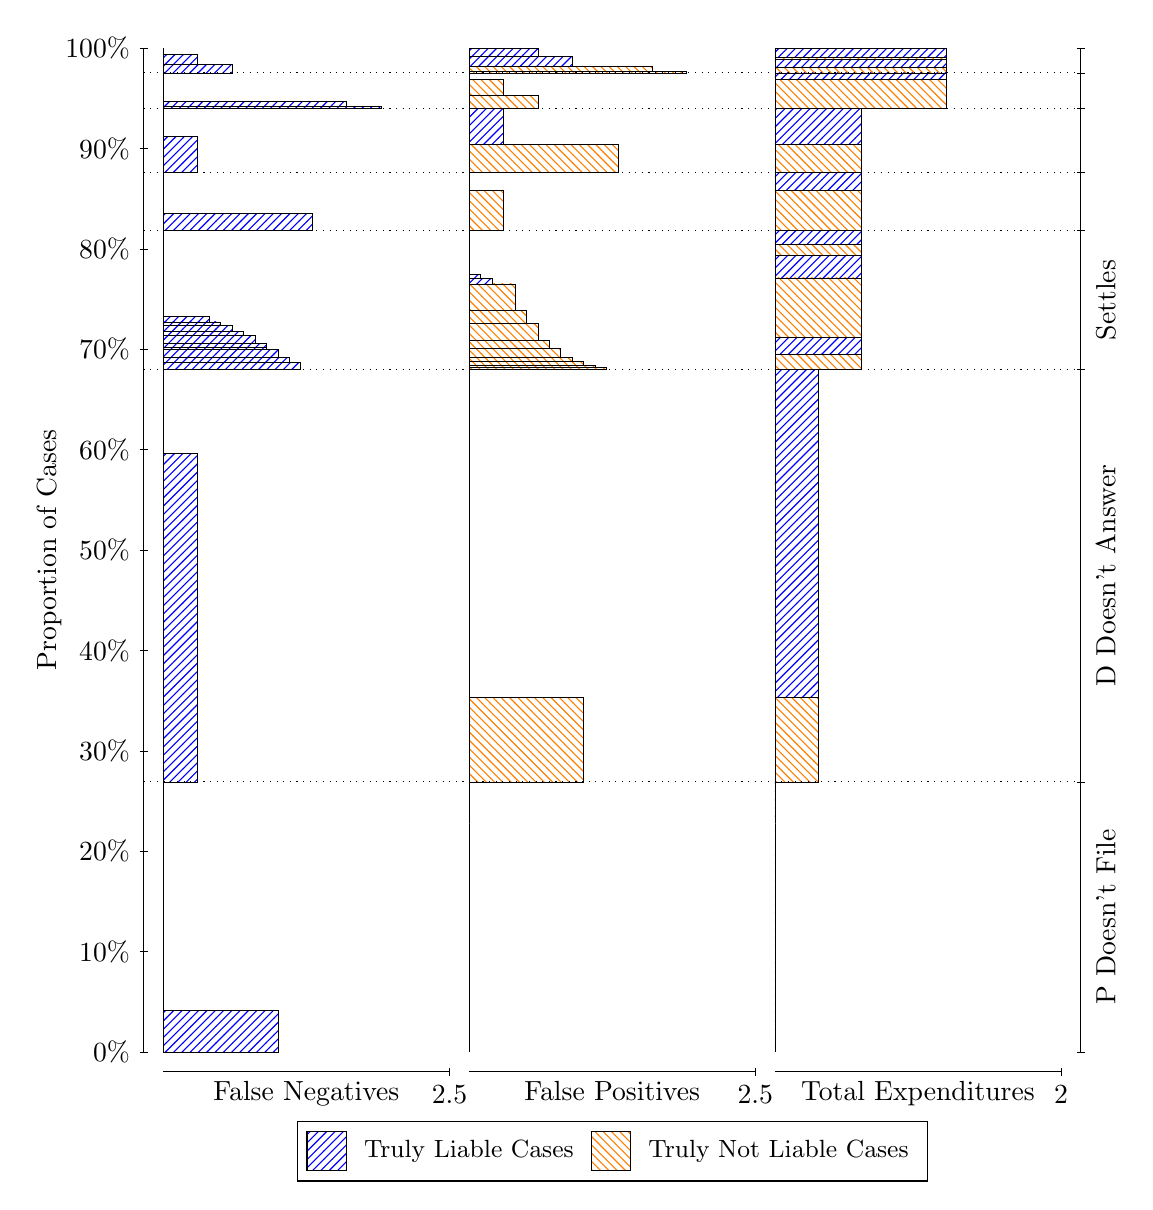
\begin{tikzpicture}
\draw[black, very thin] (1.5,1.75) -- (1.5,14.5);
\node[rotate=90, text=black, anchor=center] at (0.3, 8.125) {Proportion of Cases};
\draw[black, very thin] (1.45,1.75) -- (1.55,1.75);
\node[text=black, anchor=east] at (1.45, 1.75) {0\%};
\draw[black, very thin] (1.45,3.025) -- (1.55,3.025);
\node[text=black, anchor=east] at (1.45, 3.025) {10\%};
\draw[black, very thin] (1.45,4.3) -- (1.55,4.3);
\node[text=black, anchor=east] at (1.45, 4.3) {20\%};
\draw[black, very thin] (1.45,5.575) -- (1.55,5.575);
\node[text=black, anchor=east] at (1.45, 5.575) {30\%};
\draw[black, very thin] (1.45,6.85) -- (1.55,6.85);
\node[text=black, anchor=east] at (1.45, 6.85) {40\%};
\draw[black, very thin] (1.45,8.125) -- (1.55,8.125);
\node[text=black, anchor=east] at (1.45, 8.125) {50\%};
\draw[black, very thin] (1.45,9.4) -- (1.55,9.4);
\node[text=black, anchor=east] at (1.45, 9.4) {60\%};
\draw[black, very thin] (1.45,10.675) -- (1.55,10.675);
\node[text=black, anchor=east] at (1.45, 10.675) {70\%};
\draw[black, very thin] (1.45,11.95) -- (1.55,11.95);
\node[text=black, anchor=east] at (1.45, 11.95) {80\%};
\draw[black, very thin] (1.45,13.225) -- (1.55,13.225);
\node[text=black, anchor=east] at (1.45, 13.225) {90\%};
\draw[black, very thin] (1.45,14.5) -- (1.55,14.5);
\node[text=black, anchor=east] at (1.45, 14.5) {100\%};

\draw[black, very thin] (13.4,1.75) -- (13.4,14.5);
\draw[black, very thin] (13.35,1.75) -- (13.45,1.75);
\node[anchor=west] at (13.35, 1.75) {};
\draw[black, very thin] (13.35,5.1799) -- (13.45,5.1799);
\node[anchor=west] at (13.35, 5.1799) {};
\draw[black, very thin] (13.35,10.421) -- (13.45,10.421);
\node[anchor=west] at (13.35, 10.421) {};
\draw[black, very thin] (13.35,12.18) -- (13.45,12.18);
\node[anchor=west] at (13.35, 12.18) {};
\draw[black, very thin] (13.35,12.917) -- (13.45,12.917);
\node[anchor=west] at (13.35, 12.917) {};
\draw[black, very thin] (13.35,13.735) -- (13.45,13.735);
\node[anchor=west] at (13.35, 13.735) {};
\draw[black, very thin] (13.35,14.185) -- (13.45,14.185);
\node[anchor=west] at (13.35, 14.185) {};
\draw[black, very thin] (13.35,14.5) -- (13.45,14.5);
\node[anchor=west] at (13.35, 14.5) {};

\draw[black, very thin, pattern color=blue, pattern=north east lines] (1.75,1.75) rectangle (3.2033,2.28);
\draw[black, very thin, pattern color=orange, pattern=north west lines] (1.75,2.28) rectangle (1.75,5.1799);
\draw[black, very thin, pattern color=blue, pattern=north east lines] (1.75,5.1799) rectangle (2.186,9.3508);
\draw[black, very thin, pattern color=orange, pattern=north west lines] (1.75,9.3508) rectangle (1.75,10.421);
\draw[black, very thin, pattern color=blue, pattern=north east lines] (1.75,10.421) rectangle (3.494,10.505);
\draw[black, very thin, pattern color=blue, pattern=north east lines] (1.75,10.505) rectangle (3.3487,10.567);
\draw[black, very thin, pattern color=blue, pattern=north east lines] (1.75,10.567) rectangle (3.2033,10.676);
\draw[black, very thin, pattern color=blue, pattern=north east lines] (1.75,10.676) rectangle (3.058,10.703);
\draw[black, very thin, pattern color=blue, pattern=north east lines] (1.75,10.703) rectangle (3.058,10.751);
\draw[black, very thin, pattern color=blue, pattern=north east lines] (1.75,10.751) rectangle (2.9127,10.847);
\draw[black, very thin, pattern color=blue, pattern=north east lines] (1.75,10.847) rectangle (2.7673,10.899);
\draw[black, very thin, pattern color=blue, pattern=north east lines] (1.75,10.899) rectangle (2.622,10.979);
\draw[black, very thin, pattern color=blue, pattern=north east lines] (1.75,10.979) rectangle (2.4767,11.022);
\draw[black, very thin, pattern color=blue, pattern=north east lines] (1.75,11.022) rectangle (2.3313,11.095);
\draw[black, very thin, pattern color=orange, pattern=north west lines] (1.75,11.095) rectangle (1.75,12.18);
\draw[black, very thin, pattern color=blue, pattern=north east lines] (1.75,12.18) rectangle (3.6393,12.402);
\draw[black, very thin, pattern color=orange, pattern=north west lines] (1.75,12.402) rectangle (1.75,12.917);
\draw[black, very thin, pattern color=blue, pattern=north east lines] (1.75,12.917) rectangle (2.186,13.379);
\draw[black, very thin, pattern color=orange, pattern=north west lines] (1.75,13.379) rectangle (1.75,13.735);
\draw[black, very thin, pattern color=blue, pattern=north east lines] (1.75,13.735) rectangle (4.5113,13.76);
\draw[black, very thin, pattern color=blue, pattern=north east lines] (1.75,13.76) rectangle (4.0753,13.819);
\draw[black, very thin, pattern color=orange, pattern=north west lines] (1.75,13.819) rectangle (1.75,14.185);
\draw[black, very thin, pattern color=blue, pattern=north east lines] (1.75,14.185) rectangle (2.622,14.294);
\draw[black, very thin, pattern color=blue, pattern=north east lines] (1.75,14.294) rectangle (2.186,14.417);
\draw[black, very thin, pattern color=orange, pattern=north west lines] (1.75,14.417) rectangle (1.75,14.5);
\draw[black, very thin, pattern color=orange, pattern=north west lines] (5.6333,1.75) rectangle (5.6333,4.6499);
\draw[black, very thin, pattern color=blue, pattern=north east lines] (5.6333,4.6499) rectangle (5.6333,5.1799);
\draw[black, very thin, pattern color=orange, pattern=north west lines] (5.6333,5.1799) rectangle (7.0867,6.2503);
\draw[black, very thin, pattern color=blue, pattern=north east lines] (5.6333,6.2503) rectangle (5.6333,10.421);
\draw[black, very thin, pattern color=orange, pattern=north west lines] (5.6333,10.421) rectangle (7.3773,10.445);
\draw[black, very thin, pattern color=orange, pattern=north west lines] (5.6333,10.445) rectangle (7.232,10.47);
\draw[black, very thin, pattern color=orange, pattern=north west lines] (5.6333,10.47) rectangle (7.0867,10.519);
\draw[black, very thin, pattern color=orange, pattern=north west lines] (5.6333,10.519) rectangle (6.9413,10.569);
\draw[black, very thin, pattern color=orange, pattern=north west lines] (5.6333,10.569) rectangle (6.796,10.681);
\draw[black, very thin, pattern color=orange, pattern=north west lines] (5.6333,10.681) rectangle (6.6507,10.788);
\draw[black, very thin, pattern color=orange, pattern=north west lines] (5.6333,10.788) rectangle (6.5053,11.006);
\draw[black, very thin, pattern color=orange, pattern=north west lines] (5.6333,11.006) rectangle (6.36,11.166);
\draw[black, very thin, pattern color=orange, pattern=north west lines] (5.6333,11.166) rectangle (6.2147,11.506);
\draw[black, very thin, pattern color=blue, pattern=north east lines] (5.6333,11.506) rectangle (5.924,11.578);
\draw[black, very thin, pattern color=blue, pattern=north east lines] (5.6333,11.578) rectangle (5.7787,11.622);
\draw[black, very thin, pattern color=blue, pattern=north east lines] (5.6333,11.622) rectangle (5.6333,12.18);
\draw[black, very thin, pattern color=orange, pattern=north west lines] (5.6333,12.18) rectangle (6.0693,12.695);
\draw[black, very thin, pattern color=blue, pattern=north east lines] (5.6333,12.695) rectangle (5.6333,12.917);
\draw[black, very thin, pattern color=orange, pattern=north west lines] (5.6333,12.917) rectangle (7.5227,13.273);
\draw[black, very thin, pattern color=blue, pattern=north east lines] (5.6333,13.273) rectangle (6.0693,13.735);
\draw[black, very thin, pattern color=orange, pattern=north west lines] (5.6333,13.735) rectangle (6.5053,13.896);
\draw[black, very thin, pattern color=orange, pattern=north west lines] (5.6333,13.896) rectangle (6.0693,14.101);
\draw[black, very thin, pattern color=blue, pattern=north east lines] (5.6333,14.101) rectangle (5.6333,14.185);
\draw[black, very thin, pattern color=orange, pattern=north west lines] (5.6333,14.185) rectangle (8.3947,14.204);
\draw[black, very thin, pattern color=orange, pattern=north west lines] (5.6333,14.204) rectangle (7.9587,14.269);
\draw[black, very thin, pattern color=blue, pattern=north east lines] (5.6333,14.269) rectangle (6.9413,14.391);
\draw[black, very thin, pattern color=blue, pattern=north east lines] (5.6333,14.391) rectangle (6.5053,14.5);
\draw[black, very thin, pattern color=orange, pattern=north west lines] (9.5167,1.75) rectangle (9.5167,4.6499);
\draw[black, very thin, pattern color=blue, pattern=north east lines] (9.5167,4.6499) rectangle (9.5167,5.1799);
\draw[black, very thin, pattern color=orange, pattern=north west lines] (9.5167,5.1799) rectangle (10.062,6.2503);
\draw[black, very thin, pattern color=blue, pattern=north east lines] (9.5167,6.2503) rectangle (10.062,10.421);
\draw[black, very thin, pattern color=orange, pattern=north west lines] (9.5167,10.421) rectangle (10.607,10.608);
\draw[black, very thin, pattern color=blue, pattern=north east lines] (9.5167,10.608) rectangle (10.607,10.829);
\draw[black, very thin, pattern color=orange, pattern=north west lines] (9.5167,10.829) rectangle (10.607,11.581);
\draw[black, very thin, pattern color=blue, pattern=north east lines] (9.5167,11.581) rectangle (10.607,11.863);
\draw[black, very thin, pattern color=orange, pattern=north west lines] (9.5167,11.863) rectangle (10.607,12.007);
\draw[black, very thin, pattern color=blue, pattern=north east lines] (9.5167,12.007) rectangle (10.607,12.18);
\draw[black, very thin, pattern color=orange, pattern=north west lines] (9.5167,12.18) rectangle (10.607,12.695);
\draw[black, very thin, pattern color=blue, pattern=north east lines] (9.5167,12.695) rectangle (10.607,12.917);
\draw[black, very thin, pattern color=orange, pattern=north west lines] (9.5167,12.917) rectangle (10.607,13.273);
\draw[black, very thin, pattern color=blue, pattern=north east lines] (9.5167,13.273) rectangle (10.607,13.735);
\draw[black, very thin, pattern color=orange, pattern=north west lines] (9.5167,13.735) rectangle (11.697,14.101);
\draw[black, very thin, pattern color=blue, pattern=north east lines] (9.5167,14.101) rectangle (11.697,14.185);
\draw[black, very thin, pattern color=orange, pattern=north west lines] (9.5167,14.185) rectangle (11.697,14.25);
\draw[black, very thin, pattern color=blue, pattern=north east lines] (9.5167,14.25) rectangle (11.697,14.359);
\draw[black, very thin, pattern color=orange, pattern=north west lines] (9.5167,14.359) rectangle (11.697,14.378);
\draw[black, very thin, pattern color=blue, pattern=north east lines] (9.5167,14.378) rectangle (11.697,14.5);
\draw[black, dotted] (1.5,5.1799) -- (13.4,5.1799);
\draw[black, dotted] (1.5,10.421) -- (13.4,10.421);
\draw[black, dotted] (1.5,12.18) -- (13.4,12.18);
\draw[black, dotted] (1.5,12.917) -- (13.4,12.917);
\draw[black, dotted] (1.5,13.735) -- (13.4,13.735);
\draw[black, dotted] (1.5,14.185) -- (13.4,14.185);
\draw[black, very thin] (1.75,1.5) -- (5.3833,1.5);
\node[text=black, anchor=north] at (3.5667, 1.5) {False Negatives};
\draw[black, very thin] (5.3833,1.45) -- (5.3833,1.55);
\node[text=black, anchor=north] at (5.3833, 1.45) {2.5};

\draw[black, very thin] (5.6333,1.5) -- (9.2667,1.5);
\node[text=black, anchor=north] at (7.45, 1.5) {False Positives};
\draw[black, very thin] (9.2667,1.45) -- (9.2667,1.55);
\node[text=black, anchor=north] at (9.2667, 1.45) {2.5};

\draw[black, very thin] (9.5167,1.5) -- (13.15,1.5);
\node[text=black, anchor=north] at (11.333, 1.5) {Total Expenditures};
\draw[black, very thin] (13.15,1.45) -- (13.15,1.55);
\node[text=black, anchor=north] at (13.15, 1.45) {2};

\node[text=black, centered, rotate=90] at (13.72, 3.4649) {P Doesn't File};
\node[text=black, centered, rotate=90] at (13.72, 7.8006) {D Doesn't Answer};
\node[text=black, centered, rotate=90] at (13.72, 11.3) {Settles};





\draw (7.449999999999999,1.5) node[draw=none] (baseCoordinate) {};
\begin{scope}[align=center]
        \matrix[scale=0.5, draw=black, below=0.5cm of baseCoordinate, nodes={draw}, column sep=0.1cm]{
            \node[rectangle, draw, minimum width=0.5cm, minimum height=0.5cm, pattern color=blue, pattern=north east lines] {}; &
            \node[draw=none, font=\small, text=black] (B) {Truly Liable Cases}; &
            \node[rectangle, draw, minimum width=0.5cm, minimum height=0.5cm, pattern color=orange, pattern=north west lines] {}; &
            \node[draw=none, font=\small, text=black] (B) {Truly Not Liable Cases}; \\
            };
\end{scope}

\end{tikzpicture}
\end{document}